\chapter{MARCO TEÓRICO}

En esta sección se abordará los antecedentes de la investigacion relacionadas con herramientas de inteligencia artificial como la visión por computadora, también se incluirán las metodologías y resultados por cada artículo. Adicional, las bases teoricas y el marco conceptual. 


\section{Antecedentes de la investigación}

Los siguientes antecedentes incluyen el resumen, la metodogía y los resultados de papers de revistas y páginas importantes como National Institutes of Health (NIH) y IEEE Xplore Digital Library 

\subsection{Paper 1: A review on vision-based analysis for automatic dietary assessment (2022)}

Los autores son Wang, W., Min, W., Li, T., Dong, X. \& Li, H. de la universidades de Beijing en diferentes carreras, \parencite{wang2022review}

\textbf{Resumen}

\thinspace
Tener una dieta saludable evita problemas de salud a largo plazo, pero algunos métodos para su evaluación suelen ser poco confiables, esto a ido cambiando con la ayuda de la inteligencia artificial, este artículo presenta una arquitectura de Evaluación Dietética Basada en Visión (VBDA) que toma imágenes de una comida como entrada para luego usar visión por computadora e identificar automáticamente información dietética relevante como salida. También se evalúa la arquitectura de múltiples etapas y la de extremo a extremo. Donde la primera, arquitectura de múltiples etapas, consta de tres 3 etapas (análisis de imágenes de alimentos, estimación de volumen y derivación de nutrientes)

\textbf{Metodología}

\thinspace
La arquitectura de múltiples etapas para la Evaluación Dietética Basada en Visión (VBDA) consta de tres fases: análisis de imágenes de alimentos, estimación de porciones y derivación de nutrientes. En el caso del rendimiento de las dos primeras etapas depende de los algoritmos de IA y de los conjuntos de datos, mientras que la última, de base de datos de composición nutricional, como se muestra en la figura \ref{fig1}


\begin{figure}[h]
		\begin{center}
			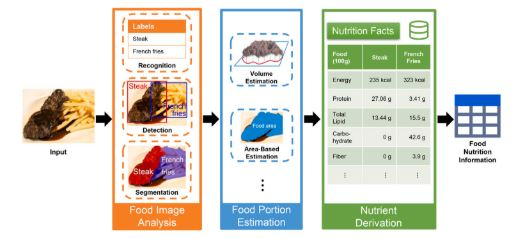
\includegraphics[width=0.8\textwidth]{2/imagen2/6FIGURA6PAPER2.JPG}
			\caption{Arquitectura de múltiples etapas}
			\label{fig1}
		\end{center}
		
	\end{figure}

\thinspace

El análisis de imágenes implica el reconocimiento, detección y segmentación de alimentos, donde el reconocimiento predice el tipo de alimento, la detección localiza y clasifica cada alimento mediante cuadros delimitadores, y la segmentación asigna etiquetas de alimentos a nivel de píxel, proporcionando una localización más precisa para la estimación de porciones, como muestra la figura \ref{fig2}

\begin{figure}[h]
		\begin{center}
			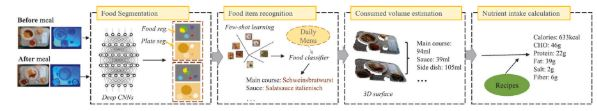
\includegraphics[width=0.8\textwidth]{2/imagen2/8FIGURA8PAPER2.JPG}
			\caption{Evaluación dietética en múltiples etapas}
			\label{fig2}
		\end{center}
		
	\end{figure}

\thinspace

En la arquitectura de extremo a extremo para la Evaluación Dietética Basada en Visión (VBDA) reemplaza múltiples etapas prácticas con una única red neuronal, reduciendo así la propagación y acumulación de errores, mejorando así la precisión y simplificando la optimización conjunta, evitando la necesidad de definir y optimizar etapas separadas con sus respectivas entradas y salidas. Además, de basarse en datos como el volumen de los alimentos, y adopta un marco multitarea para la estimación de nutrientes, abarcando componentes como proteínas y grasas, como se muestra en la figura \ref{fig3}
 
\begin{figure}[h]
		\begin{center}
			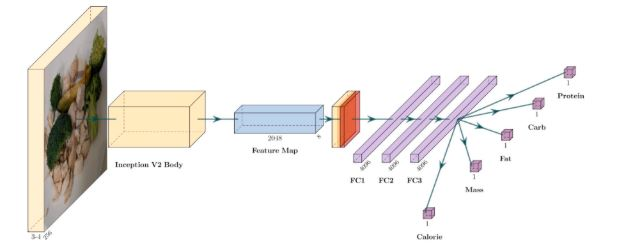
\includegraphics[width=0.8\textwidth]{2/imagen2/7FIGURA7PAPER2.JPG}
			\caption{Evaluación dietética de extremo a extremo}
			\label{fig3}
		\end{center}
		
	\end{figure}

\thinspace
También se usaron métodos para la detección de alimentos en la evaluación dietética implica la localización y reconocimiento de varios alimentos, utilizando técnicas avanzadas como Faster R-CNN y Mask R-CNN para mejorar la eficiencia y precisión del modelo. Estos métodos permiten reducir el área de reconocimiento y manejar propuestas regionales de manera más efectiva, facilitando la estimación de porciones y nutrientes. 

\thinspace

\textbf{Resultados y conclusiones}

\thinspace
La precisión del análisis visual y la estimación del volumen afecta significativamente la precisión de los resultados. En la estimación de volumen, el desempeño de la porción actual de estimación del volumen aún no es satisfactorio y obtener anotaciones precisas de las porciones y la nutrición es costoso por lo que se limita la escala de los conjuntos de datos de VBDA. Aun con ello con los datos recolectados se obtuvo un MAE de 0,0933 sobre estimación de calorías, un chi-cuadrado de 0,73 en estimación de proteínas, en el caso de reconocimiento. 

\subsection{Paper 2: A Comprehensive Survey of Image-Based Food Recognition and Volume Estimation Methods for Dietary Assessment (2021)}

Los autores son Tahir, G. \& Loo, C. del departamento de Inteligencia Artificial, Facultad de Ciencias de la Computación y Tecnología de la Información, Universidad de Malaya, Kuala Lumpur. \parencite{tahir2021comprehensive}

\textbf{Resumen}

\thinspace
Problemas como la obesidad, la hipertensión y diabetes tipo 2 se deben principalmente a una mala alimentación y estilo de vida, aunque existen aplicaciones que te ayuden con ello, suelen ser complicados ya que presentan impresiones por multidimensional, la ambigüedad entre las clases por problemas de reconocimiento de los diferentes alimentos que pueden parecer similares, también están los alimentos ocultos y la calidad de cámara, dando como resultados un bajo rendimiento de los modelos para su reconocimiento. Este artículo muestra las metodologías más efectivas para el reconocimiento de alimentos y su volumen utilizando variantes de redes neuronales convolucionales (CNN) de diferentes artículos. Como el mejorar las representaciones de imágenes de alimentos se utilizan características como la forma, color, textura como métodos visuales, también reducen la complejidad eliminando características redundantes y para el volumen el proceso en su mayoría implica de dos pasos, múltiples imágenes o una sola imagen de una cámara móvil y el cálculo del volumen de alimentos a partir de una construcción 3D o un objeto de calibración. El alcance y taxonomía de este estudio se muestra el gráfico de la figura \ref{fig4}

\begin{figure}[h]
		\begin{center}
			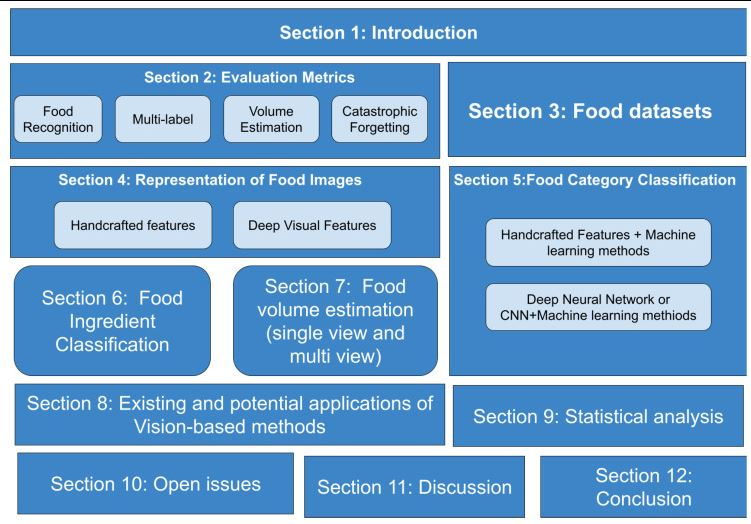
\includegraphics[width=0.6\textwidth]{2/imagen2/1FIGURA1PAPER1.JPG}
			\caption{Alcance de este estudio}
			\label{fig4}
		\end{center}
		
	\end{figure}

\thinspace
\textbf{Metodología}

\thinspace
Para la categorización de alimentos en su mayoría de artículos revisados se utilizaron métricas de evaluación como la matriz de confusión, Exactitud, Precisión, Recall, F1 Score. Para la representación de imágenes de alimentos se utilizaron principalmente dos métodos Handcrafted Features y Deep Visual Feature. En Handcrafted Features se extraen propiedades de las imágenes por algoritmos diseñados manualmente con el fin de capturar información relevante como la textura, forma y color de los alimentos, como lo muestra la figura \ref{fig5}. En Deep Visual Features, se usaron los siguiente clasificadores para el reconocimiento de imágenes de alimentos: máquinas de vectores de soporte (SVM), aprendizaje de núcleo múltiple (MKL) y K-vecino más cercano (KNN).

\begin{figure}[h]
		\begin{center}
			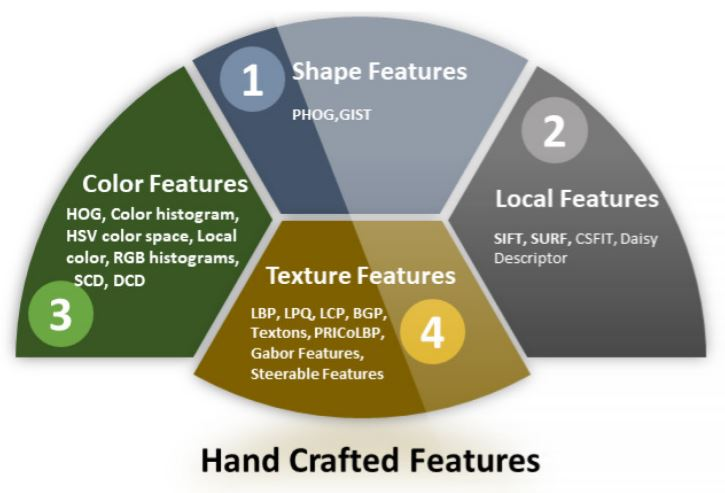
\includegraphics[width=0.7\textwidth]{2/imagen2/2FIGURA2PAPER1.JPG}
			\caption{métodos de extracción: Handcrafted feature}
			\label{fig5}
		\end{center}
		
	\end{figure}

\thinspace

Para la estimación del volumen de alimentos se categoriza como método de “vista de una sola imagen” y de “vista de múltiples imágenes/vídeo”, como muestra la figura \ref{fig6}

\begin{figure}[h]
		\begin{center}
			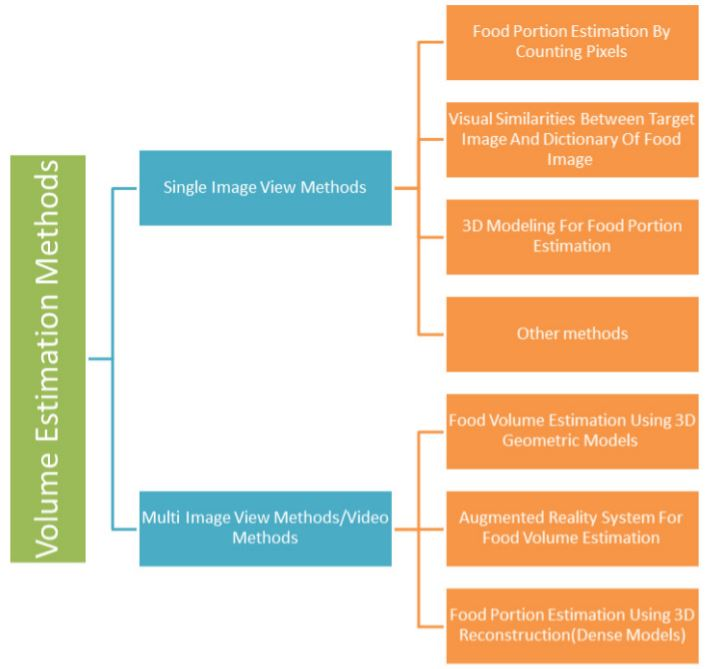
\includegraphics[width=0.7\textwidth]{2/imagen2/3FIGURA3PAPER1.JPG}
			\caption{categorizacion de estimacion de volumen}
			\label{fig6}
		\end{center}
		
	\end{figure}

\thinspace

El método de vista de imagen única para estimar el volumen de alimentos requiere solo de una imagen, por lo que son más fáciles de usar, pero son menos precisos. En cambio el de vista de múltiples imágenes, es más preciso, pero más complicado de usar debido a las múltiples imágenes desde diferentes ángulos que usan para proporcionar mejores resultados. 
\thinspace

\textbf{Resultados y conclusiones}

\thinspace
Las técnicas visuales profundas muestran un mayor rendimiento en la clasificación de alimentos, en el caso de la estimación de volúmenes de alimentos es posible calcular de manera precisa el tamaño de las porciones. Para el caso de reconocimiento de alimentos se usaron procesos como la adquisición, extracción, selección de características relevantes y la elección de la técnica de clasificación, como en la figura \ref{fig7}

\begin{figure}[h]
		\begin{center}
			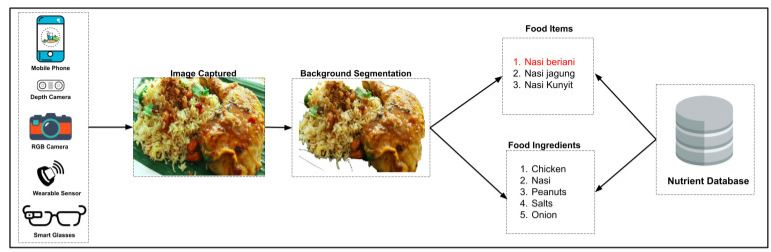
\includegraphics[width=0.7\textwidth]{2/imagen2/5FIGURA5PAPER1.JPG}
			\caption{Flujo del sistema}
			\label{fig7}
		\end{center}
		
	\end{figure}

\thinspace

 Los artículos muestran que el 38.1\% de los conjuntos de datos son genéricos, y el 46.2\% implementan CNN para el reconocimiento de alimentos. Para estimar el volumen de alimento se recomienda usar el de vista múltiple, en la figura \ref{fig8} se muestra la comparación de métodos de vista múltiple para la estimación del volumen de alimentos. 
 
\begin{figure}[h]
		\begin{center}
			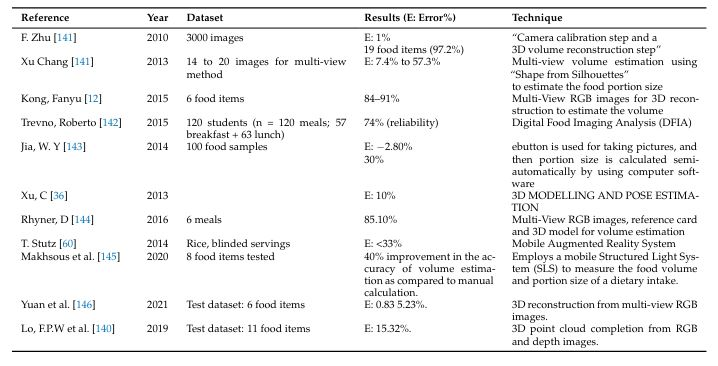
\includegraphics[width=0.7\textwidth]{2/imagen2/4FIGURA4PAPER1.JPG}
	        \caption{Comparación de métodos multivista para la estimación del volumen}
			\label{fig8}
		\end{center}
		
	\end{figure}

\thinspace

\subsection{Paper 3: DeepFood: Food Image Analysis and Dietary Assessment via Deep Model (2020)}

Los autores son Jiang, L., Bojia Q., Liu, X., Huang, C. \& Lin, K de la Facultad de Ciencias de la Computación, Universidad McGill, Montreal, Canadá, \parencite{jiang2020deepfood}

\textbf{Resumen}

\thinspace
Los avances en las herramientas de evaluación dietética y análisis nutricional mejoran la salud alimenticia, hay maneras de comprender los hábitos alimentarios diarios, explorando patrones nutricionales y promoviendo una dieta saludable. En este estudio, se muestra un sistema de evaluación dietética y reconocimiento de alimentos por aprendizaje profundo diseñado para analizar alimentos a partir de imágenes de comidas captadas por teléfonos inteligentes, por medio de tres pasos. 

Primero, se detectan las regiones candidatas en las imágenes utilizando una red de propuesta de región (RPN) derivada del modelo Faster R-CNN, segundo, estas regiones se mapean en características y se clasifican en diferentes categorías utilizando una red neuronal convolucional profunda (CNN), lo que permite su identificación en las imágenes originales. Finalmente, el sistema analiza el contenido nutricional de los alimentos reconocidos, calculando parámetros como calorías, grasas, carbohidratos y proteínas para después generar un informe de evaluación dietética. Se utilizaron dos conjuntos de datos de imágenes de alimentos conocidos (UEC-FOOD100 y UEC-FOOD256), además de introducir un nuevo conjunto de datos basado en FOOD101. Este modelo muestra una alta precisión en el reconocimiento de alimentos y genera informes de evaluación, brindando a los usuarios información valiosa sobre hábitos alimentarios saludables para una mejor salud y bienestar corporal a través de elecciones dietéticas informadas.
\thinspace

\textbf{Metodología}

\thinspace
El sistema basado en aprendizaje profundo en la detección de alimentos y se analiza los componentes nutricionales de cada imagen de comida, figura \ref{fig9}, el cual consta de tres pasos:

• Primero se extrae las regiones de interés (ROI) aplicando la red de propuesta de región derivada del modelo Faster R-CNN, con ello se separa los alimentos del fondo y mejora la eficiencia del modelo de detección.

• Segundo, se aplica una red neuronal convolucional (CNN) y se clasifica en diferentes categorías de alimentos, también se utiliza un módulo de regresión para localizar las coordenadas de los alimentos en la imagen.

• Tercero, se utilizan herramientas de evaluación dietética para el análisis de la nutrición de los alimentos y generar un informe de salud.

\begin{figure}[h]
		\begin{center}
			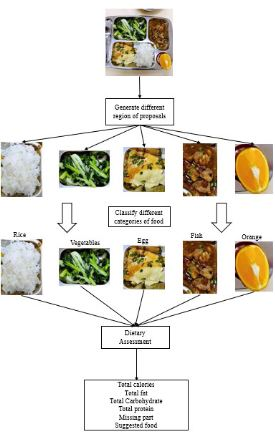
\includegraphics[width=0.5\textwidth]{2/imagen2/9FIGURA9PAPER3.JPG}
	        \caption{Reconocimiento de alimentos y análisis nutricional.}
			\label{fig9}
		\end{center}
		
	\end{figure}

\thinspace
Para la detección de alimentos, se extraen los alimentos del fondo de las imágenes y se aplica Faster R-CNN para detectar las regiones relacionadas con los alimentos. 
Para la clasificación de los alimentos, se usó la regresión del cuadro delimitador, figura \ref{fig10},  donde se ajusta el cuadro delimitador inicial para que sus coordenadas coincidan con la verdad fundamental.

\begin{figure}[h]
		\begin{center}
			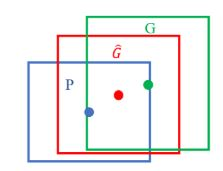
\includegraphics[width=0.2\textwidth]{2/imagen2/10FIGURA10PAPER3.JPG}
	        \caption{Regresión del Bounding box}
			\label{fig10}
		\end{center}
		
	\end{figure}

\thinspace
Para las métricas de evaluación se usó la precisión promedio media (mAP) para evaluar el modelo de detección, seguido de dos modelos: clasificación y regresión. La clasificación determina si un objeto existe en la imagen y la regresión determina la ubicación del objeto.

\thinspace
\textbf{Resultados y conclusiones}

\thinspace
En la figura \ref{fig11} se muestran los resultados en el conjunto de datos UEC-FOOD100, donde el conjunto 1 es el experimento que utilizó todas las clases de alimentos, el conjunto 2, prueba 53 clases y el conjunto 3,con 11 clases.

\begin{figure}[h]
		\begin{center}
			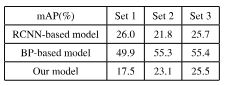
\includegraphics[width=0.5\textwidth]{2/imagen2/11FIGURA11PAPER3.JPG}
	        \caption{Los resultados en el conjunto de datos UEC-FOOD100}
			\label{fig11}
		\end{center}
		
	\end{figure}

\thinspace
En la figura \ref{fig12} se muestran los resultados en el conjunto de datos UEC-FOOD256, donde la categoría 1 es el experimento que prueba con todas las clases de alimentos, la categoría 2,con 132 clases y la categoría 3, con 21 clases.

\begin{figure}[h]
		\begin{center}
			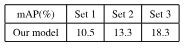
\includegraphics[width=0.5\textwidth]{2/imagen2/12FIGURA12PAPER3.JPG}
	        \caption{Los resultados en el conjunto de datos UEC-FOOD256}
			\label{fig12}
		\end{center}
		
	\end{figure}

\thinspace
Los resultados en FOOD20 con bbx se muestran en la figura \ref{fig13}.

\begin{figure}[h]
		\begin{center}
			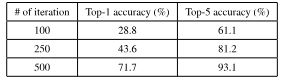
\includegraphics[width=0.5\textwidth]{2/imagen2/13FIGURA13PAPER3.JPG}
	        \caption{Los resultados en el conjunto de datos FOOD20}
			\label{fig13}
		\end{center}
		
	\end{figure}

\thinspace
Se espera mejorar la precisión de la detección, reducir el tiempo de procesamiento, y como trabajos futuros tener la predicción del peso y crear una calculadora de dieta.

\subsection{Paper 4: Image-Based Food Classification and Volume Estimation for Dietary Assessment: A Review (2020)}

Los autores son  Wen, F., Sun Y., Qiu J. \& Lo, B.. del Imperial College London, Londres, Reino Unido, publicado en el año 2020. \parencite{lo2020image}

\textbf{Resumen}

\thinspace
Existen varios métodos de evaluación dietética basados en imágenes. Este artículo compara modelos de reconocimiento de alimentos y la estimación de volumen/peso con respecto a la velocidad, precisión, eficiencia y limitaciones del procesamiento. También analiza la eficacia de métodos en el aprendizaje profundo para la evaluación dietética que combinan diferentes enfoques.

\textbf{Metodología}

\thinspace
Se usaron tres métodos para evaluar la ingesta dietética. El primero es el método de datos donde se localiza alimentos en imágenes y/o videos para reducir el almacenamiento de memoria. El segundo es el método de reconocimiento automático de alimentos, que ayuda a identificar los alimentos consumidos por los usuarios. El tercero es el método de estimación del volumen de alimentos, donde se utilizan técnicas para medir las porciones de alimento, como se muestra en la figura \ref{fig14}.

\begin{figure}[h]
		\begin{center}
			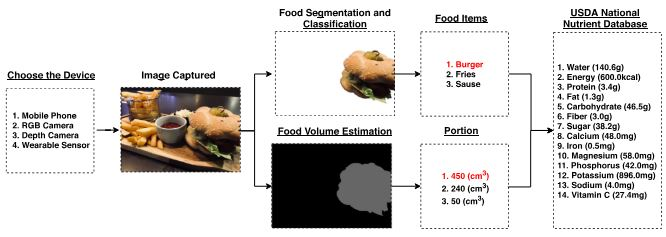
\includegraphics[width=0.5\textwidth]{2/imagen2/15FIGURA15PAPER4.JPG}
	        \caption{Diagrama del sistema para la evaluación dietética}
			\label{fig14}
		\end{center}
		
	\end{figure}

Para el reconocimiento de características de alimentos de timan en cuenta el el color, la forma y la textura, por ello hay dos enfoque principales: el reconocimiento de imágenes convencional con funciones diseñadas manualmente y el reconocimiento de imágenes de un extremo a otro con aprendizaje profundo.

En el caso del reconocimiento de imágenes convencional se usan técnicas de extracción de características como SIFT, HOG y LBP para extraer datos visuales. Para la calificación se utilizan técnicas como SVM lineal, ANN y Random Forests. Los sistemas en tiempo real utilizan técnicas de codificación como Fisher Vector para acelerar el reconocimiento. Para el aprendizaje profundo se usa las redes neuronales convolucionales (CNN)  y para la estimación de volumen de alimentos de usaron metodos como: Stereo-based Approach, Model-based, Depth Camera-based, Perspective Transformation y Deep learning, como se muestra en la figura \ref{fig15}

\begin{figure}[h]
		\begin{center}
			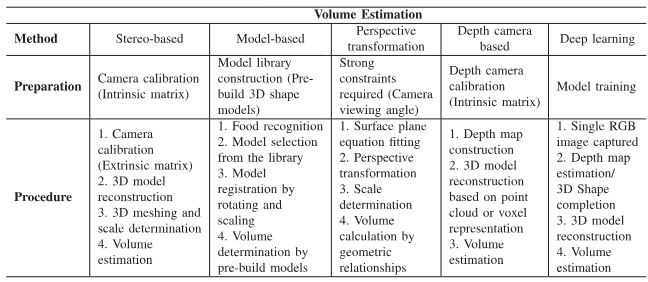
\includegraphics[width=0.5\textwidth]{2/imagen2/14FIGURA14PAPER4.JPG}
	        \caption{ Modelos para la estimación de volumen}
			\label{fig15}
		\end{center}
		
	\end{figure}

\textbf{Resultados y conclusiones}

\thinspace
La figura \ref{fig16} muestra la implementación del stereo-based volume estimation.

\begin{figure}[h]
		\begin{center}
			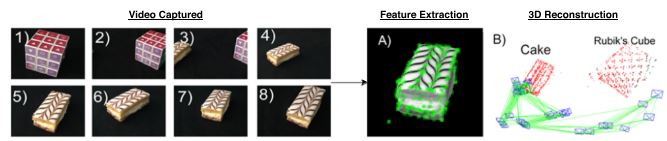
\includegraphics[width=0.5\textwidth]{2/imagen2/16FIGURA16PAPER4.JPG}
	        \caption{ implementación de la stereo-based volume estimation}
			\label{fig16}
		\end{center}
		
	\end{figure}


Los 12 mejores enfoques de aprendizaje profundo sobre clasificación de alimentos se muestran en la figura \ref{fig17}.

\begin{figure}[h]
		\begin{center}
			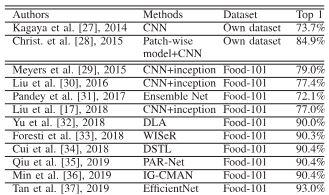
\includegraphics[width=0.5\textwidth]{2/imagen2/17FIGURA17PAPER4.JPG}
	        \caption{  Enfoques de aprendizaje profundo, TOP 12}
			\label{fig17}
		\end{center}
		
	\end{figure}

 En el reconocimiento de alimentos mediante imágenes se ha demostrado que las redes neuronales profundas superan a los enfoques tradicionales basados en características manuales. Sin embargo, persisten desafíos en la estimación de la ingesta nutricional debido al tamaño de las porciones y requieren de múltiples capturas de imágenes desde diferentes ángulos.

 \subsection{Paper 5: Deep Neural Networks for Image-Based Dietary Assessment (2021)} 

Koroušić, B. \&  Mezgec, S. del Departamento de Sistemas Informáticos Ljubljana, Eslovenia, \parencite{mezgec2021deep}.

\textbf{Resumen}

\thinspace
Con la tecnología, hoy en día, se puede registrar la ingesta con solo tomar una foto desde la cámara celular. Este artículo habla sobre el reconocimiento de alimentos en imágenes por medio de las redes neuronales profundas, utilizando la arquitectura de Nutrinet la cual es una modificación de la arquitectura AlexNet14. Aunque Nutrinet se limita a una salida de imagen de alimento,esta utiliza segmentación de imágenes ya que identifica la cantidad de alimentos y bebidas en una imagen. Los principales métodos de segmentación en este artículo son las redes totalmente convolucionales (FCN) y el otro en redes residuales profundas (ResNet). Anteriormente se ha usado extractores de características definidas manualmente pero solo han tenido precisión entre el 10\% - 40\% considerándose bajo por su apariencia variable de cada presentación de comida. Las redes neuronales convolucionales profundas (DCNN) son las más populares para el reconocimiento de imágenes de alimentos. Las capas convolucionales contienen filtros que aprenden y que responden a ciertas características de los datos de entrada, mientras que las capas completamente conectadas componen datos de salida de otras capas para obtener conocimientos de nivel superior a partir de ellos. 

\textbf{Metodología}

\thinspace
Se utilizó la arquitectura NutriNet,\ref{fig18}. Para la segmentación de imágenes se tomaron dos arquitecturas: las variaciones de las redes totalmente convolucionales (FCN-32, FCN-16 y FCN-8s15 ) y las redes residuales profundas (ResNet), como principales tomo AlexNet14, GoogLeNet y ResNet. Para el procesamiento de datos se tomó el Food Recognition Challenge y el método de Hybrid Task Cascade con ResNet-10116, también se utilizó otras redes troncales, pero se tomó la ResNet-101 como la más adecuada. Entre los parámetros de entrenamiento para tener valores óptimos se eligió el solucionador, que determina la precisión en la clasificación; la tasa de aprendizaje, donde se define la velocidad con la cambia el parámetro de la red neuronal. 

\begin{figure}[h]
		\begin{center}
			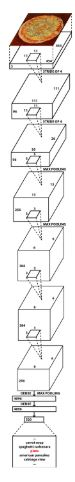
\includegraphics[width=0.05\textwidth]{2/imagen2/20FIGURA20PAPER4.JPG}
	        \caption{ Arquitectura de red neuronal profunda NutriNet}
			\label{fig18}
		\end{center}
		
	\end{figure}
 
\textbf{Resultados y conclusiones}

\thinspace
Los modelos AlexNet se entrenaron utilizando un tamaño de lote de 256 imágenes y una tasa de aprendizaje base de 0,02; NutriNet utilizó un tamaño de lote de 128 imágenes y una tasa de 0,01; GoogLeNet 64 imágenes y una tasa de 0,005; y ResNet 16 imágenes y una tasa de 0,00125, figura \ref{fig19}

\begin{figure}[h]
		\begin{center}
			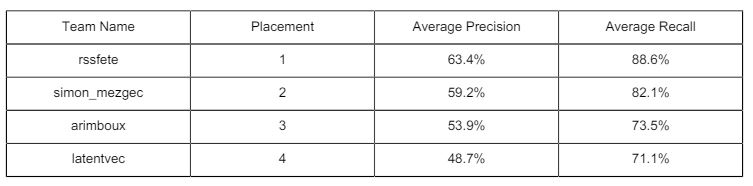
\includegraphics[width=0.7\textwidth]{2/imagen2/21FIGURA21PAPER4.JPG}
	        \caption{Reconocimiento de Alimentos}
			\label{fig19}
		\end{center}
		
	\end{figure}

Para entrenar el modelo de segmentación de imágenes de alimentos falsos del FCN-8, utilizamos Adam55. La precisión final del modelo FCN-8 entrenado fue del 92,18\%. la figura \ref{fig20} muestra, imágenes de alimentos falsos (una de cada uno de los subconjuntos de entrenamiento, validación y prueba), junto con las correspondientes etiquetas de predicción del modelo y de verdad sobre el terreno.

\begin{figure}[h]
		\begin{center}
			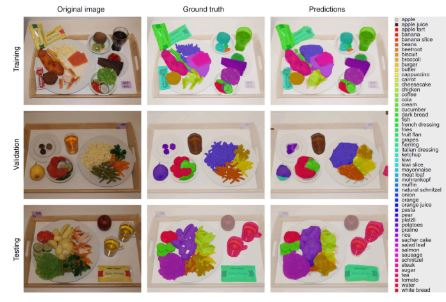
\includegraphics[width=0.5\textwidth]{2/imagen2/22FIGURA22PAPER4.JPG}
	        \caption{ Imágenes del conjunto de datos de imágenes de alimentos falsos}
			\label{fig20}
		\end{center}
		
	\end{figure}

